\textbf{Beispiel 4}\\ \\
a) \\ \\
Da sich bei B1 um eine konvexe Fläche handelt lautet der entsprechende Sichtfaktor
\[
	F_{11} = 0
\]
Da B2 die Sicht von B1 auf B3 blockiert gilt
\[
	F_{13} = 0
\]
Der Sichtfaktor zwischen B1 und B2 wird mit der Cross-String-Methode bestimmt.
\begin{figure}[h]
	\centering
	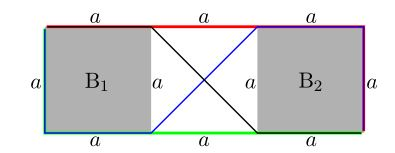
\includegraphics[width= 10cm]{tikz/17_07_2017_4a}
\end{figure}
Dieser lautet nun
\[
	F_{12} = \frac{(2a + \sqrt{2}a) + (4a + \sqrt{2}a) - 4a - 4a}{8a} = \frac{2\sqrt{2}a - 2a}{8a} = \frac{\sqrt{2} - 1}{4}
\]
Aufgrund der Geometrie gilt
\[
		F_{32} = F_{12} = \frac{\sqrt{2} - 1}{4}
\]
b) \\ \\
Mit der Summationsregel folgt
\[
	F_{14} = 1 - F_{12} = \frac{5 - \sqrt{2}}{4}
\]
Außerdem gilt durch diese Regel noch
\[
	F_{24} = 1 - F_{21} - F_{22} - F_{23}
\]
\newpage
\noindent
Da es sich bei B2 wieder um eine konvexe Fläche handelt muss wieder
\[
	F_{22} = 0
\]
gelten. Außerdem kann man aus dem Reziprozitätsgesetz
\begin{align*}
	F_{21} &= F_{12}  \\
	F_{23} &= F_{32} = F_{12}
\end{align*}
schließen. Dadurch gilt für den gesuchten Faktor
\[
	F_{24} = 1 - 2F_{12} = \frac{6 - 2\sqrt{2}}{4}
\]
Wegen der Geometrie des Problems gilt
\[
	F_{34} = F_{14} = \frac{5 - \sqrt{2}}{4}
\]
c)\\ \\
Mit dem Reziprozitätsgesetz und der Summationsregel für die benötigten Sichtfaktoren
\begin{align*}
	F_{41} &= \frac{A_1}{A_4}F_{14} = \frac{1}{6}\frac{5 - \sqrt{2}}{4} \\
	F_{42} &= \frac{A_2}{A_4}F_{24} = \frac{1}{6}\frac{6 - \sqrt{2}}{4} \\
	F_{43} &= F_{41} = \frac{1}{6}\frac{5 - \sqrt{2}}{4} \\
	F_{44} &= 1 - 2F_{41} - F_{42} = \frac{1}{6}(2 + \sqrt{2})
\end{align*}
d)\\ \\
B1 und B3 erwärmen sich schneller als B2, da die Sichtfaktoren folgendes Verhalten ausweisen.
\[
	F_{41} = F_{43} > F_{42}
\]